\documentclass[11pt]{article}
\pdfoutput=1

\usepackage{../../jcapmod}
\input{../../preamble}
\graphicspath{{figures/}}

\begin{document}
\thispagestyle{plain}

\newcommand{\errorbaricon}{%
\raisebox{-0.18ex}{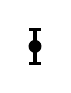
\begin{tikzpicture}[scale=1.8]
    \draw[line width=1.2pt] (0, -0.12) -- (0, 0.12);
    \draw[line width=1.2pt] (-0.04, -0.12) -- (0.04, -0.12);
    \draw[line width=1.2pt] (-0.04, 0.12) -- (0.04, 0.12);
    \fill (0, 0) circle (1.3pt);
\end{tikzpicture}}%
}

\chapterheading{\errorbaricon\hspace{0.4em}$\cdot$ Probabilistic Reasoning}

\section{Why be probabilistic?}

For years, machine learning notched wins in vision, speech, and games, while science remained largely on the sidelines. When deep learning methods finally entered scientific workflows in the late 2010s, it was probabilistic approaches that made them stick: methods that could quantify uncertainty, incorporate prior knowledge, and do more than just predict and classify. We often want to understand \emph{why} patterns exist, quantify \emph{how certain} we are, and reason about \emph{what we don't know}.

Probabilistic reasoning provides this foundation. It's the language for quantifying uncertainty in measurements and conclusions, updating beliefs as we gather evidence, comparing competing explanations for observed phenomena, and making decisions under incomplete information.
%
Every scientific conclusion rests on incomplete information. We observe a finite number of noisy measurements and try to infer something about the underlying process. Probability theory provides a consistent framework for this.

\section{Notation and probability basics}

We'll use consistent notation throughout:
\begin{itemize}
    \item $x$: \textbf{observed data}
    \item $\theta$: \textbf{parameters of interest}, the quantities we want to learn
    \item $z$: \textbf{latent variables}, unobserved quantities in the model
\end{itemize}

The notation $x \sim p(x)$ means ``$x$ is a random variable distributed according to $p$,'' or equivalently, ``$x$ is drawn from $p$.'' For example, $x \sim \mathcal{N}(\mu, \sigma^2)$ means $x$ is drawn from a Gaussian with mean $\mu$ and variance $\sigma^2$.

\paragraph{Density vs.\ probability.} For continuous variables, $p(x)$ is a \emph{probability density}, not a probability. The probability of $x$ taking any exact value is zero; instead, $p(x)\,dx$ gives the probability of $x$ falling in a tiny interval $[x, x+dx]$. Densities can exceed 1 (a narrow Gaussian has high density at its peak). To get actual probabilities, integrate: $P(a \le x \le b) = \int_a^b p(x)\,dx$. We'll use $p(\cdot)$ for both densities and probability mass functions; context makes it clear which.

\paragraph{Conditional probability.} The probability of $A$ given that we know $B$ is:
\begin{equation}
p(A \mid B) = \frac{p(A, B)}{p(B)}
\end{equation}
The intuition: conditioning on $B$ restricts our universe to only those outcomes where $B$ occurred. Within that restricted universe, $p(A \mid B)$ is the fraction where $A$ also holds: the overlap $p(A,B)$ divided by the new total $p(B)$.
This is how we update beliefs with new information.

\paragraph{Independence.} Events $A$ and $B$ are independent if $p(A, B) = p(A)p(B)$. Knowing $B$ tells us nothing about $A$. For independent observations: $p(x_1, x_2, \ldots, x_N \mid \theta) = \prod_i p(x_i \mid \theta)$.

\paragraph{Marginalization.} If we don't care about some variable, integrate it out:
\begin{equation}
p(x) = \int p(x, z)\, \d z
\end{equation}
This is how we handle nuisance parameters: integrate over them, properly propagating their uncertainty.

\begin{figure}[h]
\centering
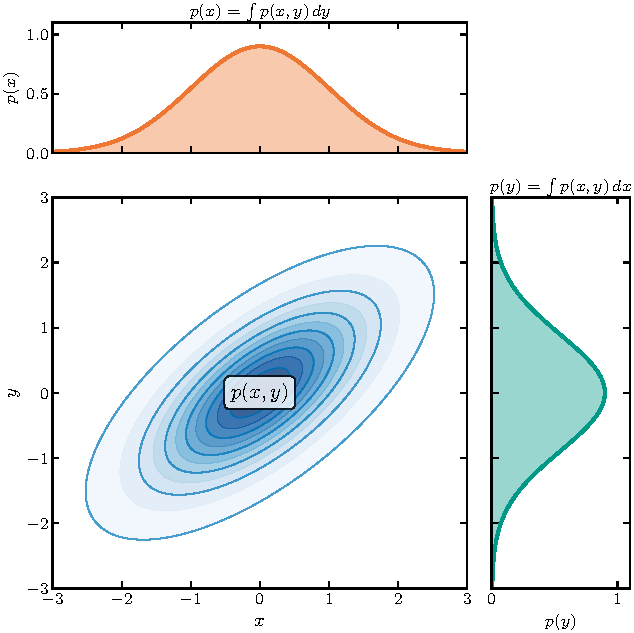
\includegraphics[width=0.5\textwidth]{marginalization.pdf}
\caption{Marginalization visualized. The central contours show a joint distribution $p(x,y)$. The marginal $p(x)$ (top) is obtained by integrating out $y$; the marginal $p(y)$ (right) by integrating out $x$.}
\label{fig:marginalization}
\end{figure}

\paragraph{Expectation values.} The expectation of a function $f(x)$ under distribution $p(x)$ is:
\begin{equation}
\E_{p(x)}[f(x)] = \int f(x) \, p(x) \, \d x
\end{equation}
This is the average value of $f$, weighted by how probable each $x$ is. Common examples: the mean is $\E[x]$, the variance is $\E[(x - \E[x])^2]$. The subscript on $\E$ clarifies which distribution we're averaging over.

\paragraph{Product rule.} Joint probabilities factor:
\begin{equation}
p(x, z) = p(x \mid z) p(z) = p(z \mid x) p(x)
\end{equation}

\paragraph{Bayes' theorem.} The product rule's symmetry gives us:
\begin{equation}
\boxed{p(\theta \mid x) = \frac{p(x \mid \theta)\, p(\theta)}{p(x)}}
\label{eq:bayes}
\end{equation}

\section{Forward vs.\ inverse problems}

This distinction is fundamental to scientific inference:

\begin{itemize}
    \item \textbf{Forward problem}: Given parameters $\theta$, sample data $x \sim p(x \mid \theta)$. This is what a simulator does: plug in masses and spins, add noise, and out comes a realization of what you might observe. The forward model is stochastic: the same parameters can produce different data due to noise, latent variables, or intrinsic randomness.

    \item \textbf{Inverse problem}: Given data $x$, infer parameters $\theta$. This is what scientific inference is all about. Inverse problems are hard, since they're ill-posed, with many parameter values consistent with the data.
\end{itemize}

The forward problem is ``easy'' in the sense that we can \emph{sample} from $p(x \mid \theta)$ by running the simulator and drawing noise. The inverse problem is hard because we need to \emph{invert} this: given one sample, characterize all the parameters (or distribution of parameters rather) that could have produced it.

\begin{figure}[h]
\centering
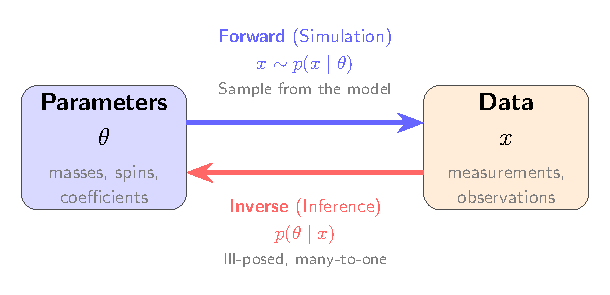
\includegraphics[width=0.85\textwidth]{forward_inverse.pdf}
\caption{Forward vs.\ inverse problems. The forward direction (simulation) samples data given parameters: $x \sim p(x \mid \theta)$. The inverse direction (inference) is ill-posed: given data, we want a distribution over parameters $p(\theta \mid x)$. Bayesian inference provides a principled framework for this inversion.}
\end{figure}

The key insight: \textbf{first specify the forward model, then invert it}. Write down how data arise from parameters, then use Bayesian inference to go backwards from observed data to parameter estimates.

\section{The data-generating process: a worked example}

Let's make this concrete with a simple example: fitting a line to noisy data.

\paragraph{Setting.} We measure $N$ data points $\{x_i\}$ at known inputs $\{t_i\}$. We believe the true relationship is linear: $x = mt + c$, but our measurements have noise. (Note: we write $x = mt + c$ rather than the conventional $y = mx + c$ to stay consistent with our notation where $x$ denotes observed data.)

\paragraph{The forward model.} We write down a story for how the data came to be:
\begin{enumerate}
    \item There are some true parameters $\theta = (m, c)$ (the slope and intercept) characterizing our model
    \item For each input $t_i$, the ``true'' value is $\mu_i = m t_i + c$
    \item We observe $x_i = \mu_i + \epsilon_i$ where $\epsilon_i \sim \mathcal{N}(0, \sigma^2)$ is measurement noise
\end{enumerate}

In probabilistic notation:
\begin{equation}
x_i \sim \mathcal{N}(m t_i + c, \sigma^2)
\end{equation}
This says: ``$x_i$ is drawn from a Gaussian distribution centered at the line, with variance $\sigma^2$.''

\begin{figure}[h]
\centering
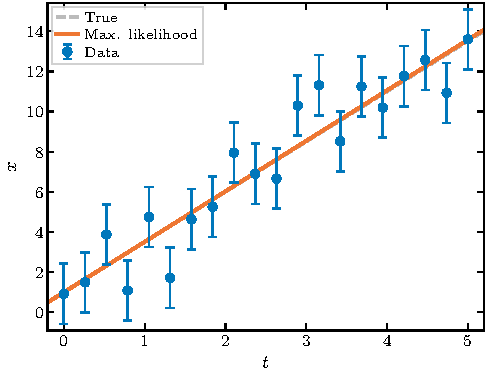
\includegraphics[width=0.5\textwidth]{line_fit_data.pdf}
\caption{Fitting a line to noisy data. Each measurement has Gaussian uncertainty $\sigma$ (shown as error bars). The gray dashed line is the true relationship; the orange line is the maximum likelihood estimate.}
\label{fig:line_fit}
\end{figure}

\section{The likelihood function}

The \textbf{likelihood} $p(x \mid \theta)$ answers: ``If the parameters were $\theta$, how probable is the observed data?''. The likelihood encodes the forward model: given parameters, predict the data distribution.
For our line-fitting example:
\begin{equation}
p(x_i \mid m, c, t_i, \sigma) = \frac{1}{\sqrt{2\pi\sigma^2}} \exp\left( -\frac{(x_i - (mt_i + c))^2}{2\sigma^2} \right)
\end{equation}

For independent observations, the joint likelihood is the product:
\begin{equation}
p(\{x_i\} \mid m, c, \{t_i\}, \sigma) = \prod_{i=1}^N p(x_i \mid m, c, t_i, \sigma)
\end{equation}

\begin{remark}
The likelihood is a function of $\theta$ (for fixed data), not a probability distribution over $\theta$. We write $\mathcal{L}(\theta) = p(x \mid \theta)$ to emphasize this. The likelihood tells us how well each $\theta$ ``explains'' the data.
\end{remark}

\section{Maximum likelihood estimation}

Before going full Bayesian, consider a simpler approach: find the parameters that make the data most probable.

\paragraph{The MLE.} The \textbf{maximum likelihood estimate} is:
\begin{equation}
\hat{\theta}_{\text{MLE}} = \arg\max_\theta p(x \mid \theta) = \arg\max_\theta \mathcal{L}(\theta)
\end{equation}

\paragraph{Log-likelihoods.} In practice, we work with log-likelihoods:
\begin{equation}
\ell(\theta) = \log p(x \mid \theta)
\end{equation}
Products become sums, which are easier numerically, and we avoid underflow when multiplying many small probabilities.

For our line example with Gaussian noise:
\begin{equation}
\ell(m, c) = -\frac{N}{2}\log(2\pi\sigma^2) - \frac{1}{2\sigma^2} \sum_{i=1}^N (x_i - mt_i - c)^2
\end{equation}
The first term is constant in $(m, c)$. Maximizing $\ell$ is equivalent to minimizing $\sum_i (x_i - mt_i - c)^2$, which is ordinary least squares.

\paragraph{Profile likelihoods.} When there are nuisance parameters, we can ``profile'' them out. For each value of the parameter of interest, maximize over nuisance parameters:
\begin{equation}
\mathcal{L}_{\text{profile}}(\theta) = \max_\phi \mathcal{L}(\theta, \phi)
\end{equation}

\begin{figure}[h]
\centering
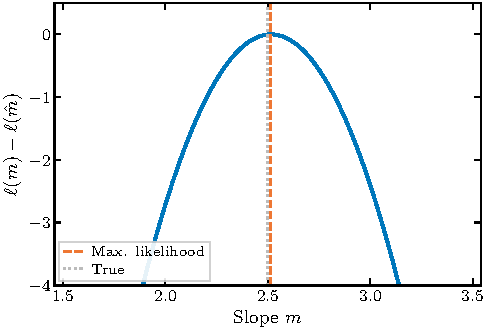
\includegraphics[width=0.5\textwidth]{profile_likelihood.pdf}
\caption{Profile likelihood for the slope parameter $m$, with the intercept $c$ profiled out. The curve shows how well each value of $m$ can fit the data (after optimizing over $c$). The peak marks the MLE of $m$.}
\label{fig:profile}
\end{figure}


\paragraph{Likelihood ratios.} Compare two hypotheses by their likelihood ratio:
\begin{equation}
\Lambda = \frac{p(x \mid \theta_1)}{p(x \mid \theta_0)}
\end{equation}
This asks: how much more probable is the data under $\theta_1$ than $\theta_0$?. Profile likelihoods let us focus on parameters of interest; likelihood ratios let us compare specific hypotheses.

\paragraph{Quantifying uncertainty.} The MLE gives a point estimate, but how certain are we? There are several frequentist approaches (confidence intervals, bootstrap, Fisher information), but we will focus on the Bayesian approach: compute the full posterior distribution.

\section{The posterior distribution}

Bayes' theorem tells us how to update beliefs:
\begin{equation}
\underbrace{p(\theta \mid x)}_{\text{posterior}} = \frac{\overbrace{p(x \mid \theta)}^{\text{likelihood}} \cdot \overbrace{p(\theta)}^{\text{prior}}}{\underbrace{p(x)}_{\text{evidence}}}
\end{equation}

\begin{itemize}
    \item $p(\theta)$ is the \textbf{prior}: what we believed before seeing data
    \item $p(x \mid \theta)$ is the \textbf{likelihood}: how probable the data is given $\theta$
    \item $p(\theta \mid x)$ is the \textbf{posterior}: what we believe after seeing data
    \item $p(x)$ is the \textbf{evidence}: a normalizing constant (more on this later)
\end{itemize}

\begin{figure}[ht]
    \centering
    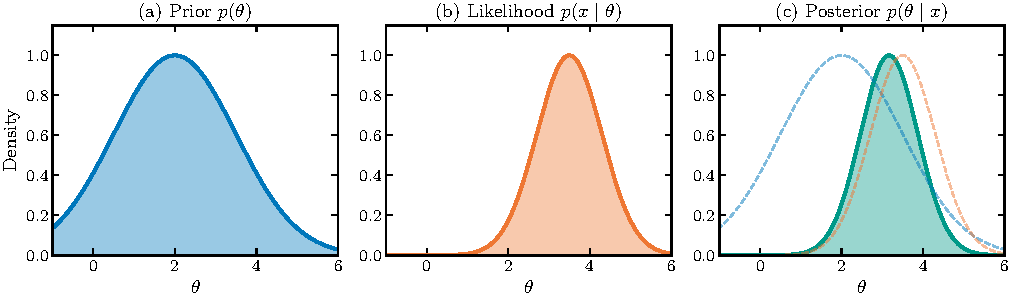
\includegraphics[width=\textwidth]{bayes_theorem.pdf}
    \caption{Bayesian inference: the prior (left) encodes initial beliefs, the likelihood (middle) peaks where data are probable, the posterior (right) combines both.}
    \label{fig:bayes}
\end{figure}

Unlike MLE which gives a point, the posterior is a \emph{distribution}. It tells us everything the data says about the parameters, given our model and prior.

\paragraph{Sequential updating.} Suppose we observe data one point at a time. After seeing $x_1$, we have posterior $p(\theta \mid x_1)$. When $x_2$ arrives, yesterday's posterior becomes today's prior:
\begin{equation}
p(\theta \mid x_1, x_2) \propto p(x_2 \mid \theta) \cdot \underbrace{p(\theta \mid x_1)}_{\text{previous posterior}}
\end{equation}
Each new observation updates our beliefs. The posterior accumulates evidence: $p(\theta \mid x_1, \ldots, x_N)$ encodes everything we've learned from all $N$ observations.

\begin{figure}[h]
\centering
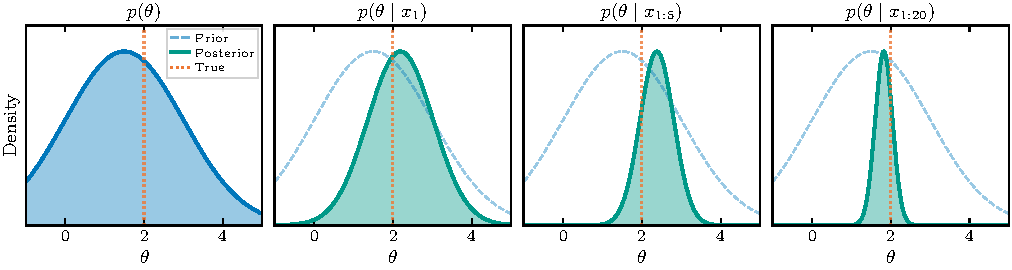
\includegraphics[width=\textwidth]{posterior_evolution.pdf}
\caption{Sequential Bayesian updating. Starting from the prior $p(\theta)$, each observation sharpens the posterior: $p(\theta) \to p(\theta \mid x_1) \to p(\theta \mid x_1, x_2) \to \cdots$. The orange dashed line marks the true value.}
\label{fig:posterior_evolution}
\end{figure}


\paragraph{Priors encode domain knowledge.} Priors are sometimes criticized as ``subjective.'' But all analysis has assumptions, and Bayesian inference makes them explicit. Priors encode physical constraints (masses must be positive), previous measurements, and reasonable ranges. This is a feature, not a bug. In well-identified problems with sufficient data, the prior's influence fades as the likelihood dominates. 

%But be aware: (1) ``flat'' priors are not parameterization-invariant (a uniform prior on $\theta$ becomes non-uniform on $\log \theta$); (2) in high dimensions, weakly identified parameters, or hierarchical models, the prior can remain influential even with large datasets.


\paragraph{Worked example.} For line fitting with a flat prior on $(m, c)$:
\begin{equation}
p(m, c \mid \{x_i\}, \{t_i\}) \propto \exp\left( -\frac{1}{2\sigma^2} \sum_{i=1}^N (x_i - mt_i - c)^2 \right)
\end{equation}
This is a 2D Gaussian! The posterior mean equals the MLE, but we also get the full covariance, including uncertainty in both parameters and their correlation.

\begin{figure}[h]
\centering
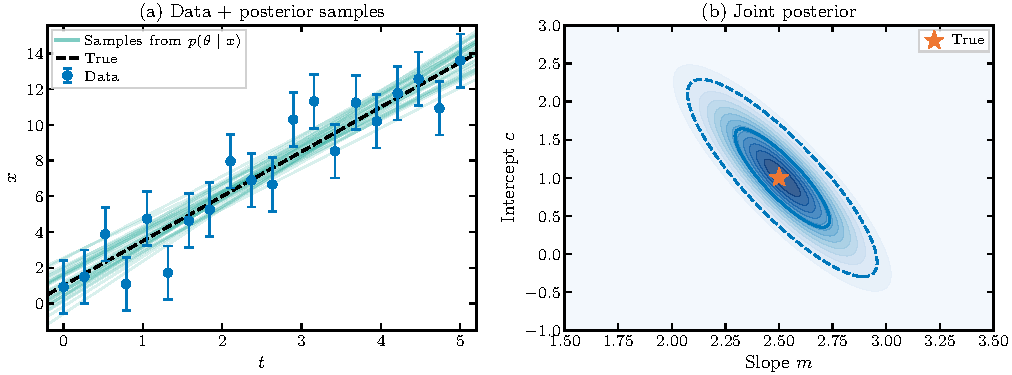
\includegraphics[width=\textwidth]{line_regression_combined.pdf}
\caption{Bayesian inference for line fitting. (a) Data with measurement uncertainties; teal lines show the range of fits consistent with the data, each a line $x = mt + c$ for a different $(m, c)$ pair drawn from the posterior. (b) Joint posterior over slope $m$ and intercept $c$, showing the characteristic anti-correlation: steeper slopes require lower intercepts.}
\label{fig:line_posterior}
\end{figure}

\paragraph{Using the posterior.} The posterior $p(\theta \mid x)$ is the complete answer, but we often need summaries:
\begin{itemize}
    \item \textbf{Point estimates}: The posterior mean $\E[\theta \mid x]$ or the mode (MAP estimate). Report one number when needed, but remember you're discarding distributional information.
    \item \textbf{Credible intervals}: A 68\% credible interval $[a, b]$ satisfies $\int_a^b p(\theta \mid x)\,\d\theta = 0.68$. The \emph{central} interval cuts off equal probability (16\%) from each tail. The \emph{highest density interval} (HDI) is the narrowest interval containing that probability---better for skewed distributions where the central interval can exclude the peak.
    \item \textbf{Marginals}: To report uncertainty on one parameter, integrate out the others: $p(\theta_1 \mid x) = \int p(\theta_1, \theta_2 \mid x)\,\d\theta_2$. The marginal propagates uncertainty including the effect of not knowing $\theta_2$.
\end{itemize}
Of course, if possible just show the full posterior!

\paragraph{Parameter degeneracy.} In Figure~\ref{fig:line_posterior}b, the posterior shows a strong anti-correlation between slope $m$ and intercept $c$: if the slope is steeper, the intercept must be lower to fit the data. This is \emph{parameter degeneracy}: different parameter combinations give similar predictions. The joint posterior captures this; looking at parameters individually would miss it.

\begin{figure}[h]
\centering
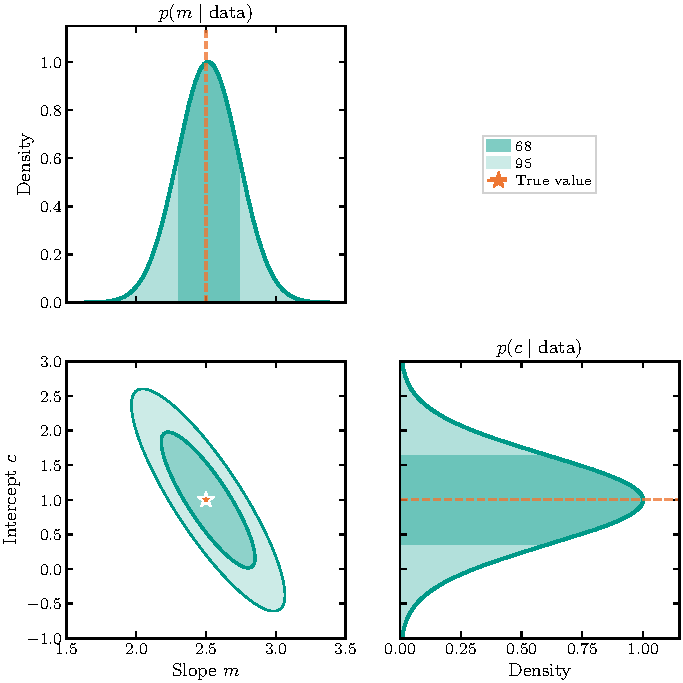
\includegraphics[width=0.65\textwidth]{corner_plot.pdf}
\caption{Corner plot for the line-fitting posterior. Diagonal: marginal distributions $p(m \mid \text{data})$ and $p(c \mid \text{data})$ with 68\% credible intervals (shaded). Off-diagonal: joint posterior with 68\% and 95\% credible regions (contours containing 68\% and 95\% of the probability mass).}
\label{fig:corner}
\end{figure}

\section{Bayesian model comparison}

We've been fitting a line to our data. But how do we know a line is the right model? Maybe the relationship is actually cubic: $y = a + bx + cx^2 + dx^3$. The cubic model can fit more patterns, but is that extra flexibility warranted?

\paragraph{The evidence.} The marginal likelihood (or ``evidence'') answers this:
\begin{equation}
p(\text{data} \mid \mathcal{M}) = \int p(\text{data} \mid \theta, \mathcal{M}) \, p(\theta \mid \mathcal{M})\, \d\theta
\end{equation}
This is the probability of the data averaged over all parameter values, weighted by the prior. It rewards models that predict the data well \emph{without} needing to tune parameters precisely.

\paragraph{Bayes factors.} To compare models, compute the ratio of evidences:
\begin{equation}
\text{BF}_{12} = \frac{p(\text{data} \mid \mathcal{M}_1)}{p(\text{data} \mid \mathcal{M}_2)}
\end{equation}
A Bayes factor of 10 means the data are 10 times more probable under model 1.

\paragraph{Example: linear vs.\ cubic.} Both models can fit our data reasonably well (Figure~\ref{fig:model_comparison}). The cubic model fits slightly better since it has more parameters to tune. But Bayes factors favor the linear model, because the cubic model's extra flexibility is wasted: it spreads its prior probability over many curves that don't match the data.

\begin{figure}[ht]
    \centering
    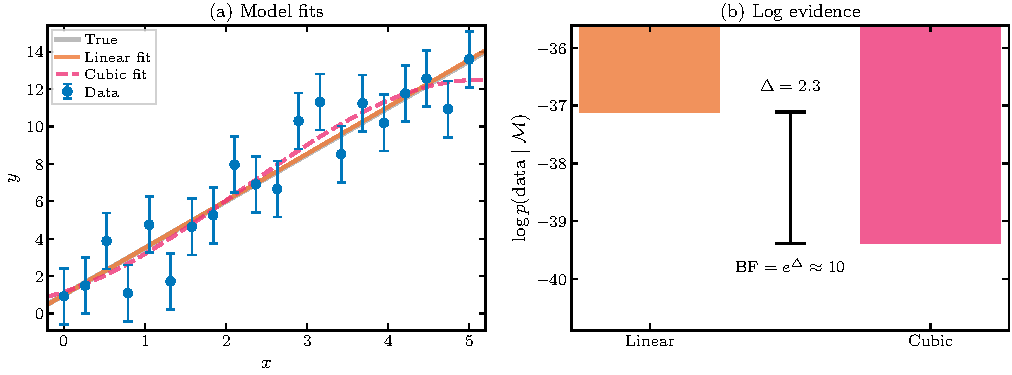
\includegraphics[width=\textwidth]{model_comparison.pdf}
    \caption{Model comparison for line-fitting data. (a) Linear ($y = a + bx$) and cubic ($y = a + bx + cx^2 + dx^3$) fits to the same data; both fit reasonably well. (b) Log evidence $\log p(\text{data} \mid \mathcal{M})$ for each model. The difference $\Delta = 2.3$ corresponds to a Bayes factor of $\approx 10$ favoring the simpler linear model.}
    \label{fig:model_comparison}
\end{figure}

\paragraph{Automatic Occam's razor.} Why does integrating over parameters penalize complexity? Figure~\ref{fig:occam} illustrates the geometric intuition. The evidence can be approximated as:
\begin{equation}
p(\text{data} \mid \mathcal{M}) \approx p(\text{data} \mid \hat{\theta}, \mathcal{M}) \times \underbrace{\frac{\text{posterior volume}}{\text{prior volume}}}_{\text{Occam factor}}
\end{equation}
A complex model with many parameters has a large prior volume, since it can fit many possible datasets. But after seeing data, the posterior concentrates in a small region. The ratio (posterior volume / prior volume) is tiny: most of the prior was ``wasted'' on parameter settings that don't match the data. A simple model has less to waste, so its Occam factor is larger. Complex models only win if they fit the data much better, enough to overcome their Occam penalty.

\begin{figure}[h]
\centering
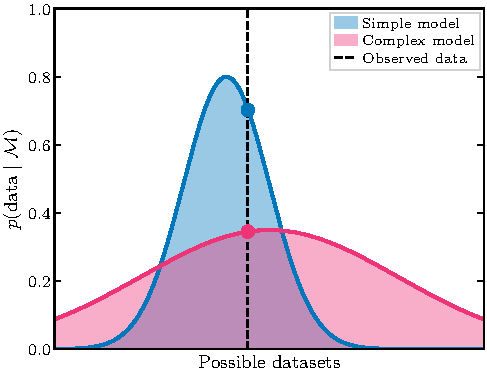
\includegraphics[width=0.5\textwidth]{model_complexity.pdf}
\caption{Bayesian Occam's razor. A simple model (blue) concentrates its prior probability in a narrow range of possible datasets, while a complex model (magenta) spreads probability over many more possibilities. At the observed data (dashed line), the simple model assigns higher probability because it ``expected'' this outcome more strongly.}
\label{fig:occam}
\end{figure}

\section{Common distributions}

A toolkit of distributions you'll encounter repeatedly. Choosing the right distribution means asking: what kind of data do I have, and what process generated it?

\paragraph{Gaussian (Normal).} $x \sim \mathcal{N}(\mu, \sigma^2)$
\begin{equation}
p(x) = \frac{1}{\sqrt{2\pi\sigma^2}} \exp\left(-\frac{(x-\mu)^2}{2\sigma^2}\right), \quad \log p(x) = -\frac{1}{2}\log(2\pi\sigma^2) - \frac{(x-\mu)^2}{2\sigma^2}
\end{equation}
Use when: measuring continuous quantities with symmetric noise. The central limit theorem says that sums of many small effects tend toward Gaussian, so it appears everywhere: measurement errors in experiments, height distributions in populations, stock price fluctuations (approximately), noise in neural recordings.

\paragraph{Poisson.} $n \sim \text{Poisson}(\lambda)$
\begin{equation}
p(n) = \frac{\lambda^n e^{-\lambda}}{n!}, \quad \log p(n) = n \log \lambda - \lambda - \log(n!)
\end{equation}
Use when: counting events that occur independently at a constant average rate $\lambda$. Examples: photon counts in astronomy, radioactive decays, website visits per hour, mutations per genome, disease cases per region. Note: for numerical stability with large $n$, compute $\log(n!)$ using the log-gamma function: $\log(n!) = \log\Gamma(n+1)$, which is available in most scientific libraries (e.g., \texttt{scipy.special.gammaln}).

\paragraph{Binomial.} $k \sim \text{Binomial}(n, p)$
\begin{equation}
p(k) = \binom{n}{k} p^k (1-p)^{n-k}, \quad \log p(k) = \log\binom{n}{k} + k \log p + (n-k) \log(1-p)
\end{equation}
Use when: counting successes in a fixed number of independent trials. Examples: coin flips, patients responding to treatment out of $n$ enrolled, defective items in a batch, correct predictions out of $n$ test cases.

\paragraph{Categorical.} $y \sim \text{Cat}(\pi_1, \ldots, \pi_K)$
\begin{equation}
p(y = k) = \pi_k, \quad \log p(y = k) = \log \pi_k, \quad \sum_k \pi_k = 1
\end{equation}
Use when: outcome is one of $K$ discrete classes. Examples: image classification (cat/dog/bird), document topics, particle types, cell types in single-cell data.

\paragraph{Uniform.} $x \sim \text{Uniform}(a, b)$
\begin{equation}
p(x) = \frac{1}{b-a}, \quad \log p(x) = -\log(b-a) \quad \text{for } x \in [a, b]
\end{equation}
Use when: all values in a range are equally plausible. Often used as a ``non-informative'' prior when you have no reason to prefer one value over another.

\paragraph{Beta.} $x \sim \text{Beta}(\alpha, \beta)$
\begin{equation}
p(x) = \frac{x^{\alpha-1}(1-x)^{\beta-1}}{B(\alpha, \beta)}, \quad \log p(x) = (\alpha-1)\log x + (\beta-1)\log(1-x) - \log B(\alpha, \beta)
\end{equation}
where $B(\alpha, \beta) = \Gamma(\alpha)\Gamma(\beta)/\Gamma(\alpha+\beta)$ is the beta function. Use when: modeling probabilities or proportions (values in $[0,1]$). The conjugate prior for Binomial success probability. $\alpha = \beta = 1$ gives Uniform; $\alpha, \beta > 1$ gives a unimodal distribution.

\paragraph{Gamma.} $x \sim \text{Gamma}(\alpha, \beta)$
\begin{equation}
p(x) = \frac{\beta^\alpha}{\Gamma(\alpha)} x^{\alpha-1} e^{-\beta x}, \quad \log p(x) = \alpha \log \beta - \log\Gamma(\alpha) + (\alpha-1)\log x - \beta x
\end{equation}
Use when: modeling positive continuous quantities (rates, variances, waiting times). The conjugate prior for Poisson rate $\lambda$. The special case $\alpha = 1$ is the Exponential distribution.

\begin{figure}[ht]
\centering
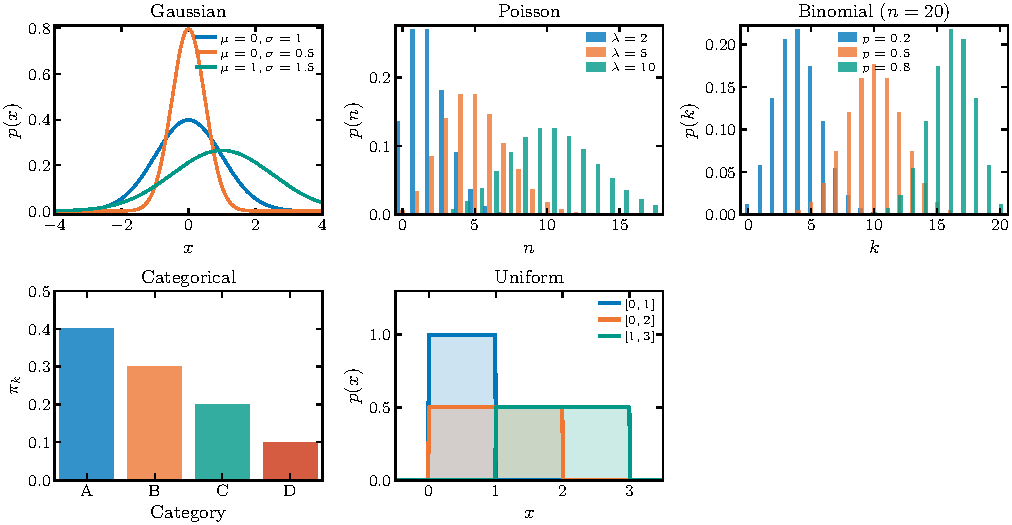
\includegraphics[width=\textwidth]{common_distributions.pdf}
\caption{Common probability distributions. Top row: Gaussian (continuous, symmetric), Poisson (discrete counts), Binomial (number of successes). Bottom row: Categorical (discrete outcomes), Uniform (flat over interval).}
\label{fig:distributions}
\end{figure}

%%%%%%%%%%%%%%%%%%%%%%%%%%%%%%%%%%%%%%%%%%%%%%%%%%%%%%%%%%%%%%%%%%
\section{Machine learning through a probabilistic lens}
%%%%%%%%%%%%%%%%%%%%%%%%%%%%%%%%%%%%%%%%%%%%%%%%%%%%%%%%%%%%%%%%%%

Every ML task is about learning a probability distribution, and we just have to figure out which one.

\subsection{What are you learning?}

You'll often see ML methods categorized as ``supervised'' vs.\ ``unsupervised.'' This is a useful organizational scheme, but it's somewhat atheoretical: it describes what labels you have, not what problem you're solving. For a science audience, the more natural framing is: What scientific question am I asking? What does my data look like? What assumptions am I encoding? The supervised/unsupervised distinction falls out of that, rather than driving it. Still, it's worth knowing the standard terminology.

\paragraph{Supervised learning: $p(x \mid t)$.} Given input-output pairs $\{(t_i, x_i)\}$, learn to predict outputs from inputs.
\begin{itemize}
    \item \textbf{Classification}: $x$ is discrete. Learn $p(x = k \mid t)$, the probability of each class given input $t$.
    \item \textbf{Regression}: $x$ is continuous. Learn $p(x \mid t)$, ideally the full distribution, not just the mean.
\end{itemize}

\paragraph{Unsupervised learning: $p(x)$.} Given only inputs $\{x_i\}$, learn the data distribution itself.
\begin{itemize}
    \item \textbf{Density estimation}: Model $p(x)$ so you can evaluate the \emph{density} (relative plausibility) of any observation. ``How typical is this galaxy image under my model?''
    \item \textbf{Generation}: Sample new $x \sim p(x)$. If you can generate realistic galaxies, you've captured something about galaxy distributions.
    \item \textbf{Anomaly detection}: Train on ``normal'' (representative) data to learn $p(x)$. Given a new observation $x^*$, compute its density $p(x^*)$. If the density is very low, the observation is unlike anything in the training set, so flag it as anomalous. Example: train on known stellar spectra, detect unusual spectra that might be new phenomena.
\end{itemize}

\paragraph{Self-supervised learning.} Use the structure of the data to create prediction tasks without external labels. Mask part of the input and predict it from the rest: $p(x_{\text{masked}} \mid x_{\text{visible}})$. Or learn that two augmented views of the same data point should have similar representations (contrastive learning). Probabilistically, you're still learning something about $p(x)$, just via a clever proxy task. This is how large language models and vision foundation models are trained. See Figure~\ref{fig:self-supervised}.

\begin{figure}[h]
\centering
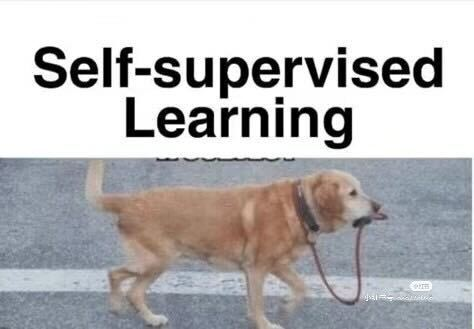
\includegraphics[width=0.55\textwidth]{self_supervised.jpg}
\caption{Look Ma, no labels.}
\label{fig:self-supervised}
\end{figure}

\paragraph{Semi-supervised learning.} You have a small labeled dataset $\{(t_i, x_i)\}$ and a large unlabeled dataset $\{x_j\}$. Use the unlabeled data to learn the structure of $p(x)$, which constrains and regularizes the supervised task. Relevant for science where labels (e.g., expensive simulations, expert annotations) are scarce but raw data is abundant.

\paragraph{Representation learning.} Learn a mapping $z = f(x)$ to a lower-dimensional latent space where useful structure is exposed. Probabilistically, this often means learning a latent variable model $p(x, z) = p(x \mid z) p(z)$ and using the inferred $z$ as a representation. The representation captures what's ``important'' about $x$ for downstream tasks. We'll go into this in detail later in the course.

\paragraph{Generative vs.\ discriminative.} This is a separate axis from supervised/unsupervised. Supervised vs.\ unsupervised asks: do you have labels? Generative vs.\ discriminative asks: do you model the data distribution? Discriminative models learn $p(\theta \mid x)$ directly: given data, predict parameters. Generative models learn $p(x \mid \theta)$, $p(x, \theta)$, or just $p(x)$. The difference matters: generative models can answer ``is this observation plausible?'' by evaluating $p(x)$. Discriminative models cannot; they only know how to map data to parameters, not whether the data makes sense.

%\begin{figure}[h]
%\centering
%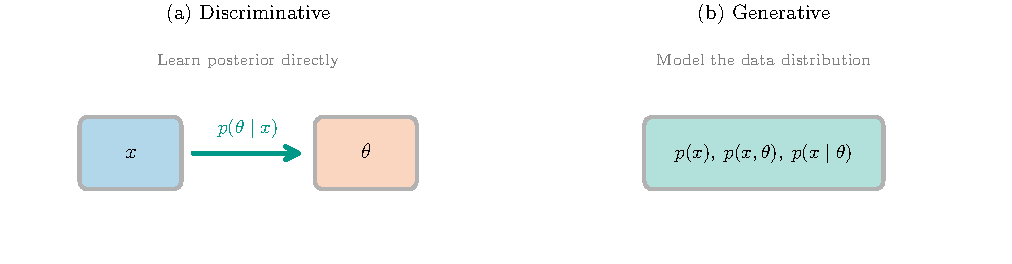
\includegraphics[width=0.8\textwidth]{generative_discriminative.pdf}
%\caption{Generative vs.\ discriminative modeling. Discriminative models learn $p(\theta \mid x)$ directly. Generative models model the data distribution: $p(x)$, the joint $p(x, \theta)$, or the conditional $p(x \mid \theta)$.}
%\label{fig:gen-disc}
%\end{figure}

\subsection{Loss functions are likelihoods}

Cross-entropy is the canonical loss for classification; MSE for regression. These aren't arbitrary choices. Every loss function encodes a probabilistic assumption, and minimizing the loss = maximizing a likelihood.

\paragraph{MSE $\Leftrightarrow$ Gaussian likelihood.} Assume observations scatter around model predictions with Gaussian noise: $x = \hat{x} + \epsilon$, where $\epsilon \sim \mathcal{N}(0, \sigma^2)$ with \emph{fixed} variance $\sigma^2$. The log-likelihood is $\log p(x \mid \hat{x}) = -\frac{1}{2\sigma^2}(x - \hat{x})^2 + \text{const}$. Since $\sigma^2$ is fixed, minimizing MSE $= \sum_i (x_i - \hat{x}_i)^2$ is equivalent to maximizing Gaussian likelihood. (If you want to learn $\sigma^2$ too, you'd need to optimize the full log-likelihood including the normalization term.)

\paragraph{Cross-entropy $\Leftrightarrow$ categorical likelihood.} For classification with $K$ classes, the categorical likelihood of observing class $c$ is $p(x = c \mid \hat{\pi}) = \hat{\pi}_c$, where $\hat{\pi}_k$ is the model's predicted probability for class $k$. If we encode the true class as a one-hot vector $x$ (with $x_c = 1$ and $x_k = 0$ for $k \neq c$), we can write $p(x \mid \hat{\pi}) = \prod_k \hat{\pi}_k^{x_k}$. Taking the log:
\begin{equation}
\log p(x \mid \hat{\pi}) = \sum_k x_k \log \hat{\pi}_k
\end{equation}
The cross-entropy loss is the negative of this: $\mathcal{L}_{\text{CE}} = -\sum_k x_k \log \hat{\pi}_k$. Minimizing cross-entropy is equivalent to maximizing the categorical log-likelihood.

\paragraph{Binary cross-entropy (BCE).} For binary classification ($K=2$), let $y \in \{0, 1\}$ be the true label and $\hat{p}$ the model's predicted probability of class 1. The BCE loss is:
\begin{equation}
\mathcal{L}_{\text{BCE}} = -y \log \hat{p} - (1-y) \log(1 - \hat{p})
\end{equation}
This is the negative log-likelihood of a Bernoulli distribution with parameter $\hat{p}$, and is a special case of cross-entropy with $K=2$.

\subsection{What's next: computing posteriors}

We now know \emph{what} we want: the posterior $p(\theta \mid x)$. But computing it requires evaluating integrals like $p(x) = \int p(x \mid \theta) p(\theta)\,\d\theta$, which are intractable in high dimensions. The next chapter covers \emph{how} to approximate these integrals:
\begin{itemize}
    \item \textbf{MCMC} (Markov chain Monte Carlo): Generate samples from the posterior by constructing a random walk that preferentially explores high-probability regions.
    \item \textbf{Variational inference}: Approximate the posterior with a simpler distribution by turning inference into optimization.
\end{itemize}
Later, we'll also see \textbf{simulation-based inference}, which learns to do inference directly from simulated data, useful when the likelihood $p(x \mid \theta)$ is hard to write down but easy to simulate.

\end{document}
